\documentclass[10pt,a4paper,headinclude,footinclude,hidelinks]{scrreprt} % KOMA-Script
\usepackage[italian]{babel}
\usepackage[utf8]{inputenc}
\usepackage[T1]{fontenc}
\usepackage{graphicx}
\usepackage{amsfonts}
\usepackage[]{../../classicthesis} % nochapters
\pagestyle{scrheadings}
\setcounter{tocdepth}{2}

\begin{document}
    \title{\rmfamily\normalfont\spacedallcaps{Modello relazionale}}
    \author{\spacedlowsmallcaps{Nicola Moretto (matr. 578258)}}
    \date{\today}
    
    \maketitle
    
    \begin{abstract}
        \noindent Il documento presenta il modello relazionale per l'integrazione dei nuovi criteri di classificazione nella piattaforma.
    \end{abstract}
    
	\begin{table}[ht]
	\centering
	\begin{tabular}{|c|c|l|}
	\hline
	\textsc{Versione} & \textsc{Data} & \textsc{Modifiche} \\ \hline
	0.1 & 2-10-2012 & Prima stesura del documento. \\ \hline
	0.2 & 3-10-2012 & Aggiunto lo \nameref{gfx:schema-relazionale}. \\ \hline
	0.3 & 3-10-2012 & Redazione della sezione \nameref{ch:stage:er:operazioni}. \\ \hline
	0.4 & 4-10-2012 & Aggiornamento e revisione della sezione \nameref{ch:stage:er:operazioni}. \\ \hline
	0.5 & 5-10-2012 & Redazione della sezione \nameref{ch:stage:er:schema}. \\ \hline
	\end{tabular}
	\caption{Registro delle modifiche}
	\label{tab:stage:wp:workload}
	\end{table}

	\tableofcontents

	%----------
	% CAPITOLO
	%----------
	\chapter{Schema relazionale}
	\label{ch:stage:er:schema}

	\begin{figure}[ht]
		\begin{center}
	    	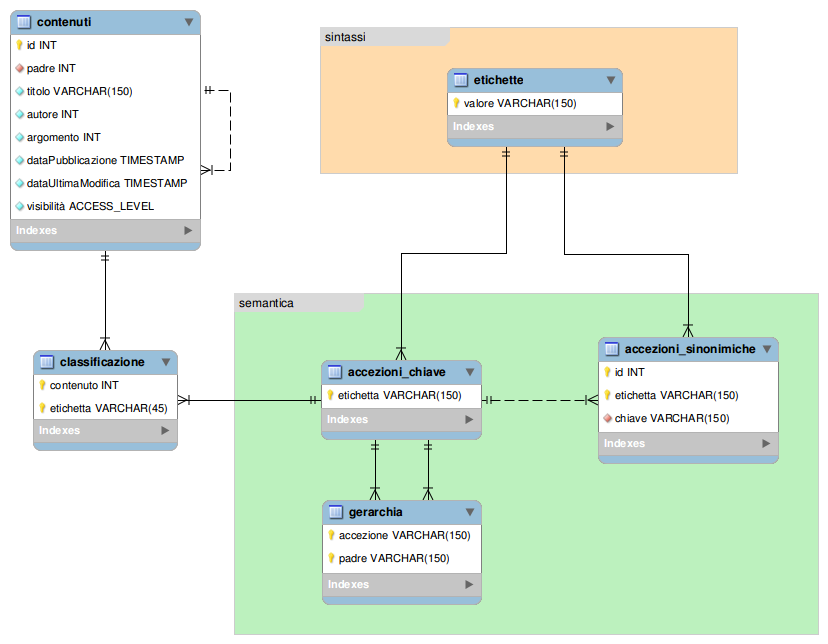
\includegraphics[width=14cm]{modello-er.png}
			\label{gfx:schema-relazionale}
			\caption{Schema relazionale del sistema di classificazione}
		\end{center}
	\end{figure}

	La progettazione dello schema relazionale\marginpar{Obiettivi} per il sistema di classificazione ha tenuto conto di diverse esigenze:
	\begin{itemize}
	\item separare le informazioni sintattiche (\textsc{etichette}) da quelle semantiche (\textsc{accezioni},\textsc{entità});
	\item evitare di dover ricorrere ad interrogazioni complesse ed onerose sul piano computazionale per reperire o inserire informazioni;
	\item garantire la massima flessibilità ed espandibilità per adattarsi alle evoluzioni tecnologiche della piattaforma (assegnazione automatica delle etichette, ricerca \textit{full-text}, \ldots).
	\end{itemize}

	\section{Sintassi}
	\subsection{etichette}
	Le etichette, intese come singole parole o brevi espressioni aventi lunghezza massima fissata (150 caratteri) e codificate secondo un formato standard, rappresentano lo strumento per identificare una determinata entità e sono a loro volta univocamente distinguibili per la struttura sintattica.

	Un'etichetta\marginpar{Accezioni} possiede diverse accezioni, ciascuna delle quali individua un'entità ben precisa del dominio e può essere chiave o sinonimica, a seconda che identifichi univocamente l'entità in questione o meno. Nel primo caso l'etichetta viene definita primaria (rispetto all'entità), altrimenti secondaria.
	
	\section{Semantica}
	\subsection{entita}
	Ciascuna entità è identificata da un'etichetta primaria, o più precisamente da un'accezione chiave di tale etichetta. La tabella \texttt{entita} rappresenta allo stesso tempo le singole entità, cui associa la corrispondente etichetta primaria, e un'accezione chiave per la medesima etichetta.

	Ciascuna etichetta può avere diverse accezioni chiave, ossia identificare univocamente diverse entità in altrettante accezioni, ma ciascuna entità ha una sola etichetta primaria.

	\subsection{tipi\textunderscore entita}
	Le entità del dominio possono essere convenientemente distinte organizzate in sotto domini a seconda di ciò che rappresentano: un luogo, una persona, un evento, un prodotto, un concetto, \ldots. 

	\subsection{sinonimi}
	Ciascuna entità è richiamabile e riferibile dall'utente mediante etichette secondarie: le accezioni secondarie di ciascuna etichetta sono presenti in tale tabella e ciascuna di esse è associata chiaramente ad un'entità del dominio.

	\subsection{gerarchia}
	Le relazioni gerarchiche tra le etichette vengono conservate in questa tabella e vengono aggiornate automaticamente in caso di aggiornamento o cancellazione di un'accezione chiave/entita.

	\section{Contenuti}
	\subsection{classificazione}
	A ciascun contenuto possono essere assegnate diverse etichette primarie, ciascuna declinata in un'accezione specifica che individua precisamente l'entità riferita nel contenuto.

	%----------
	% CAPITOLO
	%----------
	\chapter{Operazioni}
	\label{ch:stage:er:operazioni}
	In questo capitolo vengono illustrate le operazioni essenziali di gestione e utilizzo del sistema di classificazione progettato ed implementato secondo le specifiche descritte nella sezione \ref{ch:stage:er:schema}.

	Per ciascuna operazione, si descrive lo scopo e si fornisce il codice \textit{SQL} con cui realizzarle, motivando ove opportuno le scelte di progettazione del database e mostrando i vantaggi ottenuti.

	Di seguito si assume che le etichette rispettino un formato standard, a garanzia dell'assenza di duplicati; le variabili nel codice SQL, il cui valore è noto al momento dell'esecuzione dell'istruzione, sono riconoscibili dal prefisso '@'.

% TO DO
% principio di sostituzione

	% SECTION
	\section{Etichette}
	\label{ch:stage:er:operazioni:etichette}
	Le etichette rappresentano la componente sintattica mediante la quale gli utenti interagiscono con il sistema di classificazione, catalogando e recuperando i contenuti.

	\subsection{Ricerca di un'etichetta}
	\label{ch:stage:er:operazioni:etichette:ricerca}
	Una stringa digitata dall'utente può rappresentare il prefisso di un'etichetta o l'etichetta stessa: in entrambi i casi per cercare riscontri nel dizionario è sufficiente considerare la tabella \texttt{etichette}.

	\paragraph{Corrispondenza esatta} \hfill \\
	Restituisce - ove presente - l'etichetta corrispondente alla stringa inserita.

\begin{verbatim}
SELECT *
  FROM etichette
 WHERE valore='@etichetta'
\end{verbatim}

	\paragraph{Corrispondenza parziale} \hfill \\
	Restituisce - ove presenti - le etichette corrispondenti alla stringa inserita o di cui quest'ultima sia prefisso.

\begin{verbatim}
SELECT *
  FROM etichette	
 WHERE valore LIKE '@etichetta%'
\end{verbatim}

	\subsection{Ricerca delle accezioni di un'etichetta}
	\label{ch:stage:er:operazioni:etichette:accezioni}
	Individuata un'etichetta, è spesso necessario recuperare le relative accezioni per identificare un'entità precisa del dominio. Tale operazione richiede di consultare separatamente le tabelle \texttt{entita} e \texttt{sinonimi} e di unire i risultati, eventualmente ordinandoli alfabeticamente.

\begin{verbatim}
{
  SELECT id
    FROM entita	
   WHERE etichetta='@etichetta'
}
UNION
{
  SELECT entita
    FROM sinonimi	
   WHERE etichetta='@etichetta'
}
ORDER BY id
\end{verbatim}

	\subsection{Ricerca dell'etichetta primaria}
	\label{ch:stage:er:operazioni:etichette:ricerca-primaria}
	Se l'etichetta inserita dall'utente risulta - rispetto ad un'accezione - secondaria, è necessario risalire alla corrispondente primaria. Ciò richiede di consultare le tabelle \texttt{entita} e \texttt{sinonimi}: è possibile effettuare tale operazione mediante un'unica istruzione SQL, che richiede il JOIN tra le due tabelle, o due distinte.

\paragraph{Istruzione singola}
\begin{verbatim}
SELECT e.etichetta
  FROM entita AS e JOIN sinonimi AS s
       ON (e.id=s.entita)
 WHERE s.etichetta='@etichetta' AND s.id='@id'
\end{verbatim}

\paragraph{Due istruzioni}
\begin{verbatim}
SELECT entita
  FROM sinonimi	
 WHERE s.etichetta='@etichetta' AND s.id='@id'

SELECT etichetta
  FROM entita	
 WHERE c.etichetta='@entita'
\end{verbatim}

	\subsection{Ricerca del numero di assegnazioni di un'etichetta}
	\label{ch:stage:er:operazioni:etichette:occorrenze}
	Per determinare il numero di contenuti cui sia stata assegnata una data etichetta è sufficiente accedere alla tabella \texttt{classificazione}.

\begin{verbatim}
SELECT COUNT(*) AS num
  FROM classificazione
 WHERE etichetta='@etichetta'
\end{verbatim}

	\subsection{Inserimento di un'etichetta}
	\label{ch:stage:er:operazioni:etichette:inserimento}
	L'inserimento di una nuova etichetta si rende necessario qualora un utente cerchi di riferire un'entità con una stringa (parola o breve espressione) non presente nel dizionario (vedi sezione \ref{ch:stage:er:operazioni:etichette:ricerca-primaria}).

	A questo punto l'etichetta viene inserita nella tabella \texttt{etichette}:
\begin{verbatim}
INSERT INTO etichette
     VALUES (@stringa,current_timestamp)
\end{verbatim}

	Infine si deve associarle almeno un'accezione, che chiarisca l'entità cui si riferisce: tale operazione può essere svolta dall'utente o in maniera (semi)automatica, mediante l'assegnazione di valori predefiniti.\footnote{L'assegnazione automatica dell'accezione è possibile solo per la prima.}

	Di seguito si assume che l'utente abbia stabilito se si tratti di etichetta primaria (identifica una nuova entità) o secondaria (identificatore alternativo per un'entità definita), sfruttando eventualmente l'organizzazione per tipi.

	\paragraph{Accezione chiave} \hfill \\
	Se l'etichetta è primaria, si fornisce una descrizione dell'entità in questione.
\begin{verbatim}
INSERT INTO entita(etichetta,tipo)
     VALUES (@etichetta,@tipo)
\end{verbatim}

	\paragraph{Accezione sinonimica} \hfill \\
	Se l'etichetta è secondaria, è necessario indicare la corrispondente accezione chiave.
\begin{verbatim}
INSERT INTO sinonimi(etichetta,entita)
     VALUES (@etichetta,@entita)
\end{verbatim}

	\subsection{Eliminazione di un'etichetta}
	Il processo di eliminazione di un'etichetta richiede di prendere in esame ciascuna accezione ed eliminarla, secondo le modalità specificate nella sezione \ref{ch:stage:er:operazioni:accezioni:eliminazione}.

	Solo una volta cancellate le relative accezioni, è possibile procedere all'eliminazione dell'etichetta dal dizionario.
\begin{verbatim}
DELETE FROM etichette
      WHERE valore=@etichetta
\end{verbatim}

	\subsection{Calcolo di affinità tra due etichette primarie}
	L'affinità tra due etichette primarie è espressa dal numero di contenuti in cui compaiano entrambe le entità riferite.
\begin{verbatim}
  SELECT contenuto, COUNT(*)
    FROM classificazione
   WHERE entita='@entita1' OR entita='@entita2'
GROUP BY contenuto
  HAVING COUNT(*)>=2
\end{verbatim}

	% SECTION
	\section{Accezioni}
	\label{ch:stage:er:operazioni:accezioni}
	
	\subsection{Eliminazione di un'accezione}
	\label{ch:stage:er:operazioni:accezioni:eliminazione}
	L'eliminazione di un'accezione associata ad un'etichetta richiede di considerare due casi distinti, a seconda che l'accezione stessa sia chiave o sinonimica.

	\paragraph{Accezione sinonimica} \hfill \\
	In questo caso si può procedere all'eliminazione diretta, poiché l'entità in questione continua ad essere identificata da un'altra etichetta primaria (la cui accezione è chiave).
\begin{verbatim}
DELETE FROM sinonimi
      WHERE etichetta='@etichetta' AND id='@id'
\end{verbatim}

	\paragraph{Accezione chiave} \hfill \\
	In quest'altro caso, prima di procedere all'eliminazione, occorre individuare un'etichetta secondaria da rendere primaria, "promuovendo" l'accezione corrispondente da sinonimica (tabella \texttt{sinonimi}) a chiave (tabella \texttt{entita}).

	Per prima cosa si individua un'accezione sinonimica con cui sostituire l'accezione chiave (ove non ve ne sia nessuna, l'intera operazione va annullata).
\begin{verbatim}
SELECT *
  FROM sinonimi
 WHERE entita='@entita'
 LIMIT 1
\end{verbatim}

	A questo punto si sostituisce l'accezione chiave con la sinonimica, aggiornando l'etichetta assegnata alla prima con il valore della seconda. Così facendo le restanti accezioni sinonimiche riferenti la medesima entità si aggiorneranno automaticamente.
\begin{verbatim}
UPDATE entita
   SET etichetta='@etichetta_sinonimica'
 WHERE id='@entita'
\end{verbatim} 

	Infine si elimina l'accezione sinonimica.
\begin{verbatim}
DELETE FROM sinonimi
      WHERE etichetta='@etichetta_sinonimica' AND id='@id'
\end{verbatim}

	% SECTION
	\section{Entit\`a}
	Ciascuna entità è identificata univocamente nel sistema di classificazione da un'accezione chiave e - sul piano sintattico - dalla relativa etichetta primaria. Per tale motivo la maggior parte delle operazioni coinvolge le tabelle \texttt{accezioni\textunderscore chiave} e \texttt{gerarchia}.
 
	\subsection{Ricerca dei figli}
	La ricerca dei figli di un'entità consiste nell'individuare le entità di cui essa sia il padre.
\begin{verbatim}
SELECT e.etichetta AS figlio
  FROM gerarchia AS g JOIN entita AS e
       ON (g.figlio=e.id)
 WHERE padre='@entita'
\end{verbatim}

	\subsection{Ricerca dei padri}
	La ricerca dei padri di un'entità risulta analoga e simmetrica rispetto alla precedente.
\begin{verbatim}
SELECT e.etichetta AS padre
  FROM gerarchia AS g JOIN entita AS e
       ON (g.padre=e.id)
 WHERE figlio='@entita'
\end{verbatim}

	\subsection{Ricerca delle etichette}
	Per ottenere la lista completa delle etichette con cui è riferibile una determinata entità del dominio, è sufficiente recuperare l'etichetta primaria e quelle sinonimiche.

\begin{verbatim}
{
  SELECT etichetta
    FROM entita
   WHERE entita='@entita'
}
UNION
[
  SELECT etichetta
    FROM sinonimi AS s JOIN entita AS e
         ON (s.entita=e.id)
   WHERE s.entita='@entita'
}
\end{verbatim}

	\subsection{Aggiungere una relazione padre-figlio}
	L'aggiunta di un una relazione padre-figlio tra entità esistenti richiede di specificare padre e figlio nella tabella \texttt{gerarchia}.
\begin{verbatim}
INSERT INTO gerarchia(entita,padre)
     VALUES (@figlio,@padre)
\end{verbatim}

	Un controllo elementare per evidenziare l'incompatibilità della relazione tra due entità consiste nel verificare se risulti già definita una relazione ove la coppia (padre,figlio) sia scambiata. L'operazione può essere effettuata automaticamente all'inserimento della nuova riga grazie ad un trigger.
	
\begin{verbatim}
DELIMITER $
CREATE TRIGGER controlloRelazionePadreFiglioEntita
BEFORE INSERT ON classificazione
FOR EACH ROW BEGIN
  DECLARE records INT;

  SELECT COUNT(*) INTO records
    FROM classificazione
   WHERE padre=NEW.figlio AND figlio=NEW.padre;

  IF records>0 THEN
    SIGNAL SQLSTATE '45000'
    SET MESSAGE_TEXT = 'Relazione padre-figlio inversa già presente';
  END IF;
END; $
DELIMITER ;
\end{verbatim}

	% SECTION
	\section{Contenuti}
	\subsection{Assegnazione di un'etichetta}
	L'assegnazione di un'etichetta (più precisamente un'accezione chiave) ad un contenuto assume che sia stata individuata l'etichetta primaria per l'entità in questione (v. sezioni \ref{ch:stage:er:operazioni:etichette:ricerca} e \ref{ch:stage:er:operazioni:etichette:accezioni}). A questo punto si procede inserendo una nuova riga nella tabella \texttt{classificazione}.
\begin{verbatim}
INSERT INTO classificazione(contenuto,entita)
     VALUES (@contenuto,@entita)
\end{verbatim}

	\subsection{Ricerca delle etichette assegnate}
	Il reperimento della lista delle etichette primarie	assegnate ad un contenuto richiede di consultare le tabelle \texttt{classificazione} ed \texttt{entita}.
\begin{verbatim}
SELECT e.etichetta
  FROM classificazione AS c JOIN entita AS e
       ON (c.entita=e.id)
 WHERE contenuto='@contenuto'
\end{verbatim}

	%Il numero di contenuti trovati esprime l'attinenza delle etichette, ossia quanto vengano usate insieme 
	\subsection{Ricerca di contenuti generici}
	La ricerca dei contenuti cui sia stata assegnata una certa etichetta richiede di consultare la tabella \texttt{classificazione}.
\begin{verbatim}
SELECT contenuti
  FROM classificazione
 WHERE entita='@entita'
\end{verbatim}

	\subsection{Ricerca di contenuti specifici}
	La ricerca di contenuti specifici consiste nell'individuare i contenuti cui siano state assegnate - tra le altre - determinate etichette (due o più) specificate dall'utente. 
\begin{verbatim}
  SELECT contenuto, COUNT(etichetta)
    FROM classificazione
   WHERE entita='@entita1' [OR entita='@entita2' ...]
GROUP BY contenuto
  HAVING COUNT(*)>=@num_etichette
\end{verbatim}

\end{document}
